
\title{Sistemi Informativi \\ Laboratorio 3}
\author{
        Catalin Copil
            \and
        Mattia de Stefani
            \and
        Giulio Lovisotto
}
\date{\today}

\documentclass[12pt]{article}
\usepackage{algorithmicx}
\usepackage{algpseudocode}
\usepackage{graphicx}
\usepackage{geometry}



\addtolength{\topmargin}{-.5in}
\begin{document}
\maketitle

\section{Descrizione}

Abbiamo scelto di usare l'algoritmo di ranking BM25 .
Tale algoritmo funziona nel modo seguente:

\[ \sum\limits_{i \in Q}\log\Bigl(\frac{(r_i+0.5)/(R-r_i+0.5)}{(n_i-r_i+0.5)/(N-n_i-R+r_i+0.5)}\Bigl)\cdot\frac{(k_1+1)f_i}{k+f_i}\cdot\frac{(k_2+1)qf_i}{k_2+qf_i} \]

dove:
\begin{itemize}
\item $i$ sono i termini della query $Q$, 
\item $r_i$ e' il numero di documenti rilevanti che contiene il termine $i$,
\item $R$ e' il numero di documenti rilevanti per la query, 
\item $n_i$ e' il numero di documenti che contiene il termine $i$ nella collezione,
\item $N$ e' il numero totale di documenti nella collezione, 
\item $k_1, k_2$ sono parametri,
\item $f_i$ e' la frequenza del termine $i$ nel documento,
\item $qf_i$ e' la frequenza del termine $i$ nella query,
\item $K$ e' definito nel modo seguente:
\[ K = k_1((1-b) +b \cdot \frac{dl}{avdl}) \]
dove $b$ e' un parametro, $dl$ e' la lunghezza del documento, $avdl$ e' la lunghezza media di un documento nella collezione. Questo termine serve a normalizzare il componente di frequenza rispetto alla lunghezza del documento (per non favorire i documenti troppo lunghi).
\end{itemize}
I termini $R$ e $r_i$ sono informazioni note a priori, tipicamente sono settati a zero in quanto non si hanno informazioni sulla rilevanza. Nel nostro caso li ignoriamo lasciandoli a zero.

\section{Implementazione}
 
Descriviamo ora le strutture dati necessarie al reperimento che vengono calcolate durante l'indicizzazione. 
\begin{itemize}
\item matrice delle frequenze n\_docs x n\_words
\item un array che contiene le lunghezze dei documenti
\end{itemize}
La funzione di reperimento scorrera' la lista di documenti (le righe della matrice), e per ogni documento scorrera' sui termini della query $Q$ (\textit{Document-at-a-time retrieval}). Poi i documenti con punteggio maggiore di zero verranno ordinati (dal maggiore al minore). Il seguente pseudocodice mostra la procedura di retrieval:


\begin{algorithmic}
\State $Q \gets query$
\ForAll{$doc \in C$} 
    \State $score\gets 0$
    \ForAll{$qw \in Q$}
        \State $score \gets score + f_{bm25}(doc, qw)$
    \EndFor
\EndFor\\
\Return top $k$ scoring documents
\end{algorithmic}

La complessita' di tale algoritmo e' $O(n \cdot m)$ dove $n$ e' il numero di documenti nella collezione $C$, e $m$ e' il numero di descrittori nell'interrogazione $Q$. Per i parametri abbiamo scelto: $k_1=0.01$, $k_2=1$, $b=0$, in quanto fornivano la migliore precisione nei risultati. Il termine $b$ a zero significa che non viene applicato alcuno $smoothing$ sulle frequenze rispetto alla lunghezza del documento, nel nostro caso cio' funziona perche' i documenti sono in genere molto corti. Il termine $k_1$ e' stato settato ad un valore molto basso in quanto essendo i documenti molto corti (per alcuni ci sono solo 2-3 parole), la componente di frequenza nella formula di BM25 aveva un peso troppo influente rispetto alle altre.

\section{Risultati}
Abbiamo valutato i risultati della nostra implementazione con l'utility \textit{trec\_eval} e abbiamo ottenuto i risultati riportati in figura.
\begin{figure}[htbp]
\begin{center}
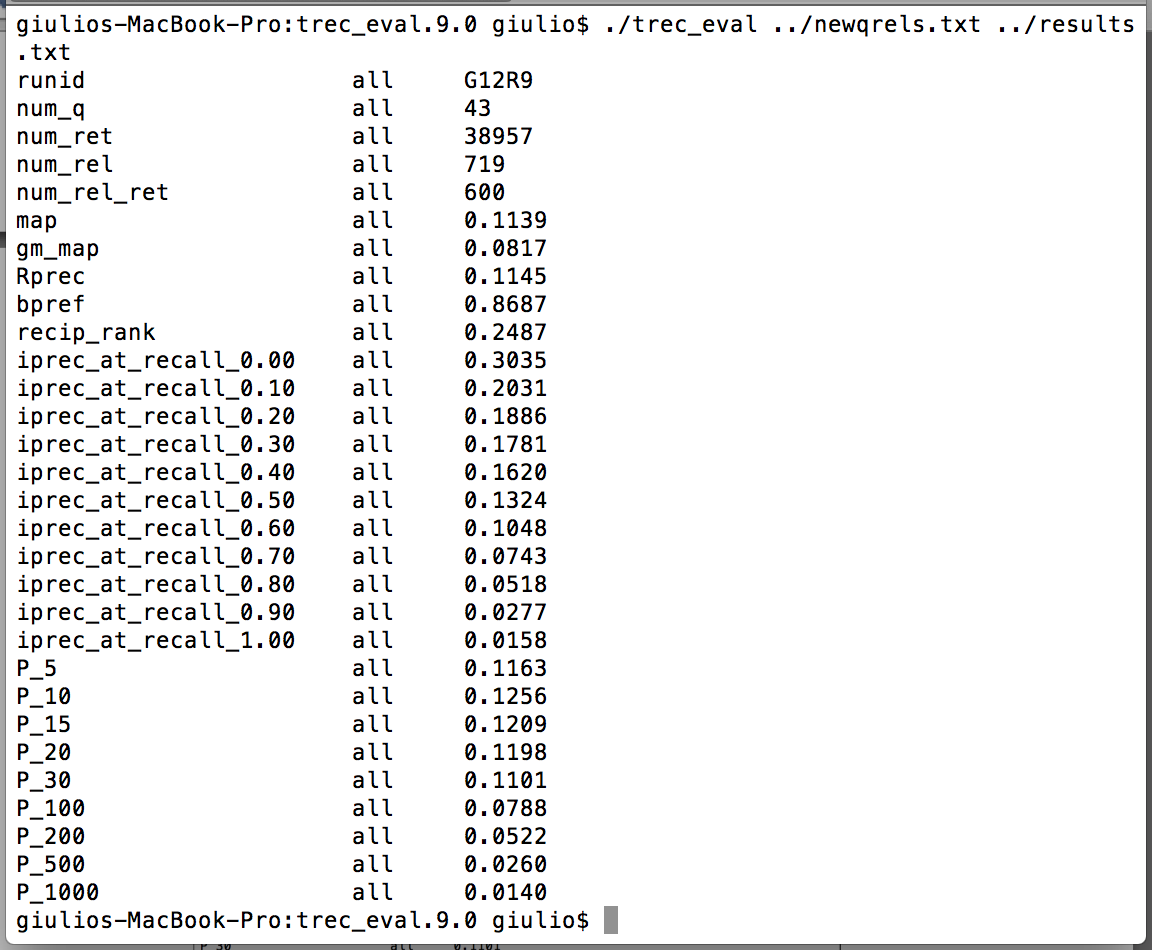
\includegraphics[width=0.75\textwidth]{myresult.png}
\caption{Risultati \textit{trec\_eval}}
\label{fig:fig1}
\end{center}
\end{figure}

Si puo' vedere che la $map$ e' piuttosto bassa. Indagando sulle query abbiamo notato che alcune di esse contengono bisogni informativi legati agli autori (``I am interested in articles written either by Prieve or Udo PoochPrieve, B. Pooch, U.''), e nella nostra implementazione cio' non e' colto in quanto nei documenti indicizzati il campo autori e' ignorato (nei file non sono presenti gli stem degli autori). Inoltre non sempre gli stem presenti nei file forniti rappresentano sempre il bisogno informativo (``Interested in articles on robotics, motion planning particularly the geometric and combinatorial aspects. We are not interested in the dynamics of arm motion.'') in quanto il modello scelto non permette di esprimere condizioni booleane.

\subsection{Lucene}
Per confrontare i risultati abbiamo utilizzato il modulo \textsc{PyLucene} (python api per lucene). Abbiamo indicizzato i seguenti campi dei documenti: autore, abstract, titolo, prendendoli dal testo originale in xml. Figura 2 riporta i risultati ottenuti.
\begin{figure}[htbp]
\begin{center}
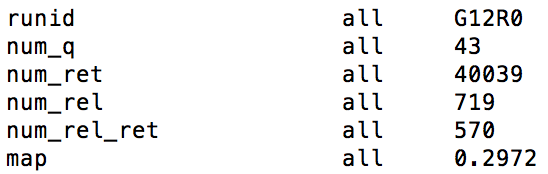
\includegraphics[width=0.75\textwidth]{result2.png}
\caption{Risultati \textit{trec\_eval} sull'output di lucene}
\label{fig:fig2}
\end{center}
\end{figure}
\bibliographystyle{abbrv}
\bibliography{main}

Come si puo' vedere la $map$ e' leggermente inferiore nonostante l'utilizzo del campo autori, che nella nostra implementazione non e' presente. Cio' e' dovuto alla funzione di ranking di lucene, che combina modello vettoriale e probabilistico ma non tiene conto della brevita' dei documenti della nostra collezione.
\end{document}